\documentclass{article}
\usepackage{graphicx}

\title{CARA MEMBUAT APLIKASI PEMINJAMAN RUANGAN POLITEKNIK POS INDONESIA MENGGUNAKAN ORACLE APEX}
\author{Nurul Kamila (1184038) }
\date{18 December 2019}

\begin{document}

\maketitle
\begin{enumerate}
    \item 	Pertama dan paling utama sekali tentu saja kita akan membuka oracle apex itu sendiri dengan mengunjungi https://apex.oracle.com, lalu sign in dengan menginputkan workspace, email/username, serta password kita.
    \begin{center}
    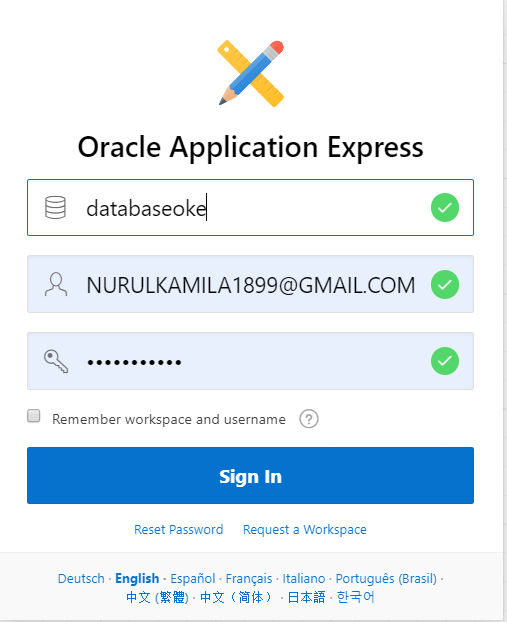
\includegraphics[width=.6\textwidth]{Figure/14.PNG}
    \end{center}
    
    \item   Kemudian, pada laman tampilan awal kita akan menemui beberapa menu seperti App Builder, SQL Workshop, Team Development, dan App Gallery
    
    \item   Pada tahap awal pembuatan aplikasi ini, kita harus membuat tabel-tabel yang akan dimasukkan dan diperlukan pada aplikasi ini. Disini saya membuat empat tabel yaitu tabel Mahasiswa1, tabel BAAK, tabel Peminjaman, dan Tabel Ruang.
    
    \item   Untuk membuat tabel tersebut klik SQL Workshop dan pilih SQL Command, lalu ketikkan queriesnya seperti dibwah ini;
     \begin{enumerate}
         \item  Tabel Mahasiswa1\\
         Pada tabel Mahasiswa1 ini akan terdapat 5 kolom, yaitu kolom NPM, Nama MHS, JURUSAN, KELAS , dan JUMLAH PEMINJAMAN. Dimana, primary key pada tabel ini adalah NPM.
         \begin{center}
         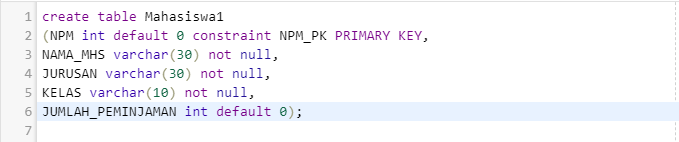
\includegraphics[width=.8\textwidth]{Figure/q1.PNG}
         \end{center}
         
         \item  Pada tabel BAAK ini akan terdapat 2 kolom, yaitu kolom ID PEGAWAI, dan NAMA PEGAWAI, dimana ID PEGAWAI merupakan primarykey dari tabel tersebut. 
         \begin{center}
         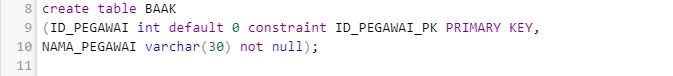
\includegraphics[width=.8\textwidth]{Figure/q2.PNG}
         \end{center}
         
         \item  Pada tabel Peminjaman ini akan terdapat 6 kolom, yaitu kolom ID PEMINJAMAN, TGL PEMINJAMAN,TGL PENGEMBALIAN, NPM, ID PEGAWAI, dan ID RUANG, dimana ID PEMINJAMAN merupakan primarykey dari tabel tersebut dan NPM, ID PEGAWAI, serta ID RUANG sebagai Foregentkeynya.
         \begin{center}
         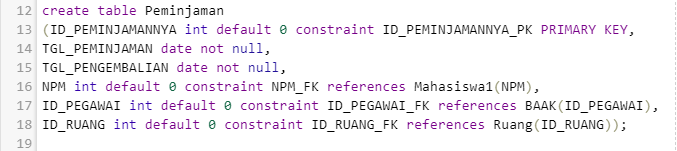
\includegraphics[width=.8\textwidth]{Figure/q3.PNG}
         \end{center}
         
         \item  Pada tabel Ruang ini akan terdapat 2 kolom, yaitu kolom ID RUANG, dan NAMA RUANGAN, dimana ID RUANG merupakan primarykey dari tabel tersebut.
         \begin{center}
         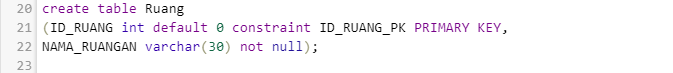
\includegraphics[width=.8\textwidth]{Figure/q4.PNG}
         \end{center}
     \end{enumerate}
     
     \item  Setelah membuat semua tabel yang diperlukan,  inputkan data sesuai masing-masing tabel tersebut, seperti contoh di bawah ini:
     \begin{enumerate}
         \item   Data pada tabel Mahasiswa1
         \begin{center}
         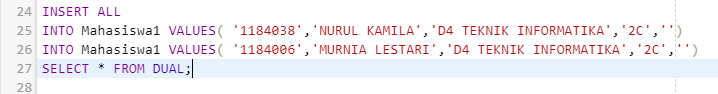
\includegraphics[width=.8\textwidth]{Figure/q5.PNG}
         \end{center}
         
         \item  Data pada tabel BAAK
         \begin{center}
         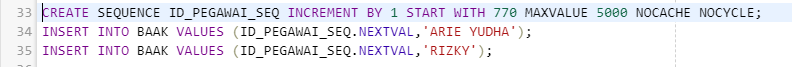
\includegraphics[width=.8\textwidth]{Figure/q6.PNG}
         \end{center}
         
         \item  Data pada tabel Peminjaman
         \begin{center}
         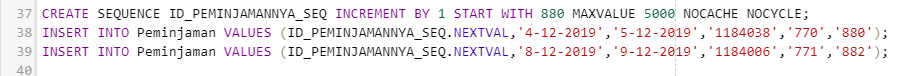
\includegraphics[width=.8\textwidth]{Figure/q7.PNG}
         \end{center}
         
         \item  Data pada tabel Ruang
         \begin{center}
         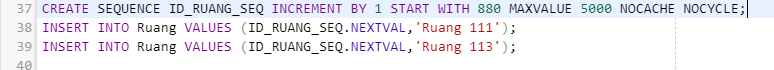
\includegraphics[width=.8\textwidth]{Figure/q8.PNG}
         \end{center}
     \end{enumerate}
     
     \item  Selanjutnya, jika kita sudah membuat tabel-tabel yang diperlukan serta menginputkan datanya sesuai masing-masing tabel, buatlah queries trigger seperti contoh di bawah ini:
     \begin{center}
     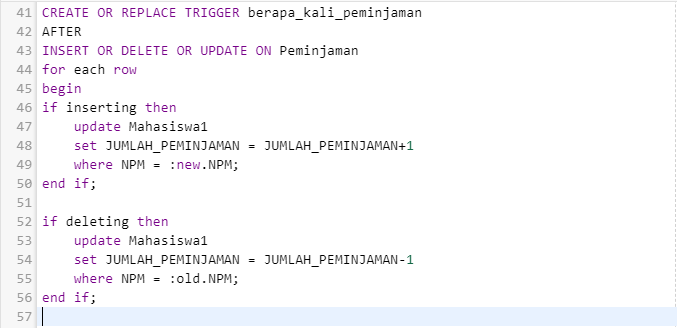
\includegraphics[width=.8\textwidth]{Figure/q9.PNG}
     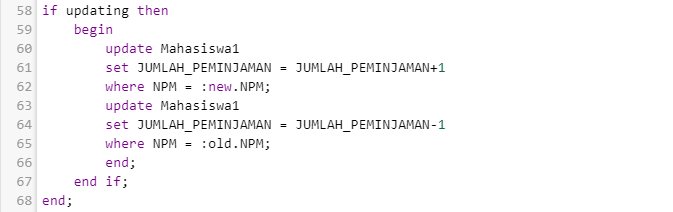
\includegraphics[width=.8\textwidth]{Figure/q9-1.PNG}
     \end{center}
     Trigger dalam database adalah kode prosedural yang secara otomatis dijalankan untuk menanggapi perubahan tertentu pada table tertentu atau tampilan dalam database. Trigger dapat didefinisikan untuk menjalankan perintah sebelum atau setelah eksekusi DML (Data Manipulation Language) seperti INSERT, UPDATE, dan DELETE.\\
     \\
     Pada queries trigger di atas, dapat di ambil kesimpulan bahwa kita akan membuat trigger \textbf{berapa kali peminjaman} yang dimana jika kita melakukan insert atau update atau delete pada tabel Peminjaman, maka nanti akan berpengaruh pada tabel Mahasiswa1 tepatnya pada kolom \textbf{JUMLAH PEMINJAMAN}, yang apabila kita melakukan insert maka data \textbf{JUMLAH PEMINJAMAN} tersebut bertambah satu, dan apabila kita melakukan delete akan berkurang satu.
     
     \item  Setelah berhasil melakukan trigger, lanjut untuk membuat queries view
     \begin{center}
     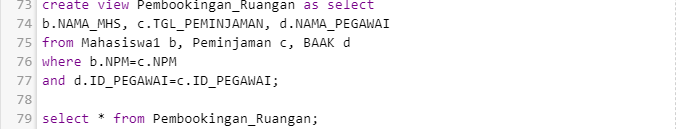
\includegraphics[width=.8\textwidth]{Figure/q10.PNG}
     \end{center}
     SQL View adalah tabel virtual (bukan tabel sebenarnya) yang dibuat dari beberapa tabel atau view lain. SQL View tidak memiliki data sendiri, tetapi data-datanya berasal dari tabel-tabel atau view lain.\\
     \\
     Pada queries view di atas, dapat kita simpulkan bahwa pada view \textbf{Pembookingan Ruangan} akan terdapat atau menampilkan kolom \textbf{Nama MHS} yang berasal atau diambil dari tabel Mahasiswa1, kolom \textbf{TGL PEMINJAMAN} yang berasal atau diambil dari tabel Peminjaman, dan kolom \textbf{NAMA PEGAWAI} yang berasal atau diambil dari tabel BAAK.
     
     \item  Jika kita ingin memanggil atau menampilkan data pada sebuah tabel dengan nama yang berbeda namun memiliki arti yang sama, kita dapat menggunakan queries synonym seperti contoh dibawah ini:
     \begin{center}
     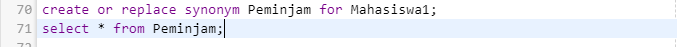
\includegraphics[width=.8\textwidth]{Figure/q11.PNG}
     \end{center}
     
     \item  Setelah kita selesai membuat tabel-tabel beserta isi datanya, dan menggunakan trigger, view, dan synonym seperti yang sudah kita lakukan diatas. Maka tahap selanjutnya yaitu mengcreate aplikasinya . Pertama kita buka menu App Builder, lalu pilih Create.
     \begin{center}
     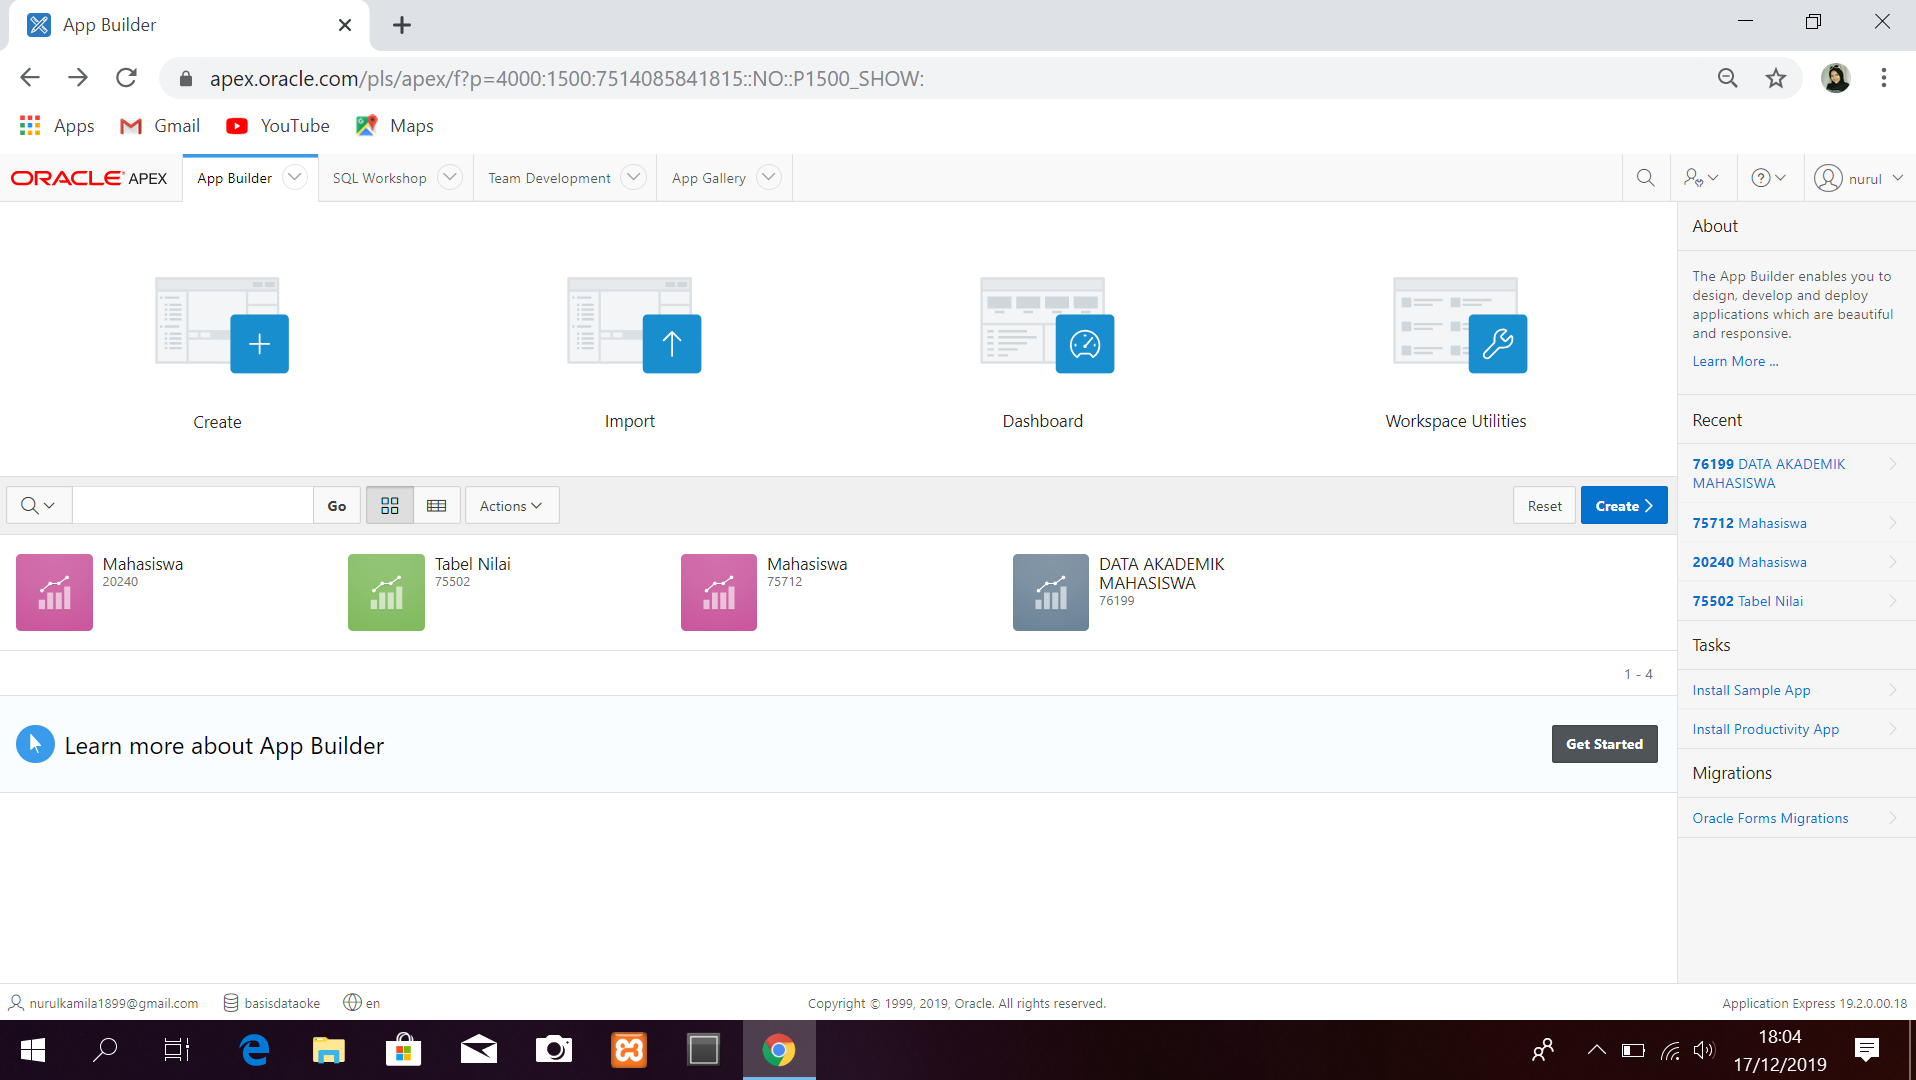
\includegraphics[width=.8\textwidth]{Figure/1.PNG}
     \end{center}
     
     \item  selanjutnya pada halaman create an application, kita akan menemui 3 pilihan yaitu New Application, From a File, dan Productivity App. Dikarenakan kita akan membuat aplikasi baru dari awal, maka disini kita memilih New Application
     \begin{center}
     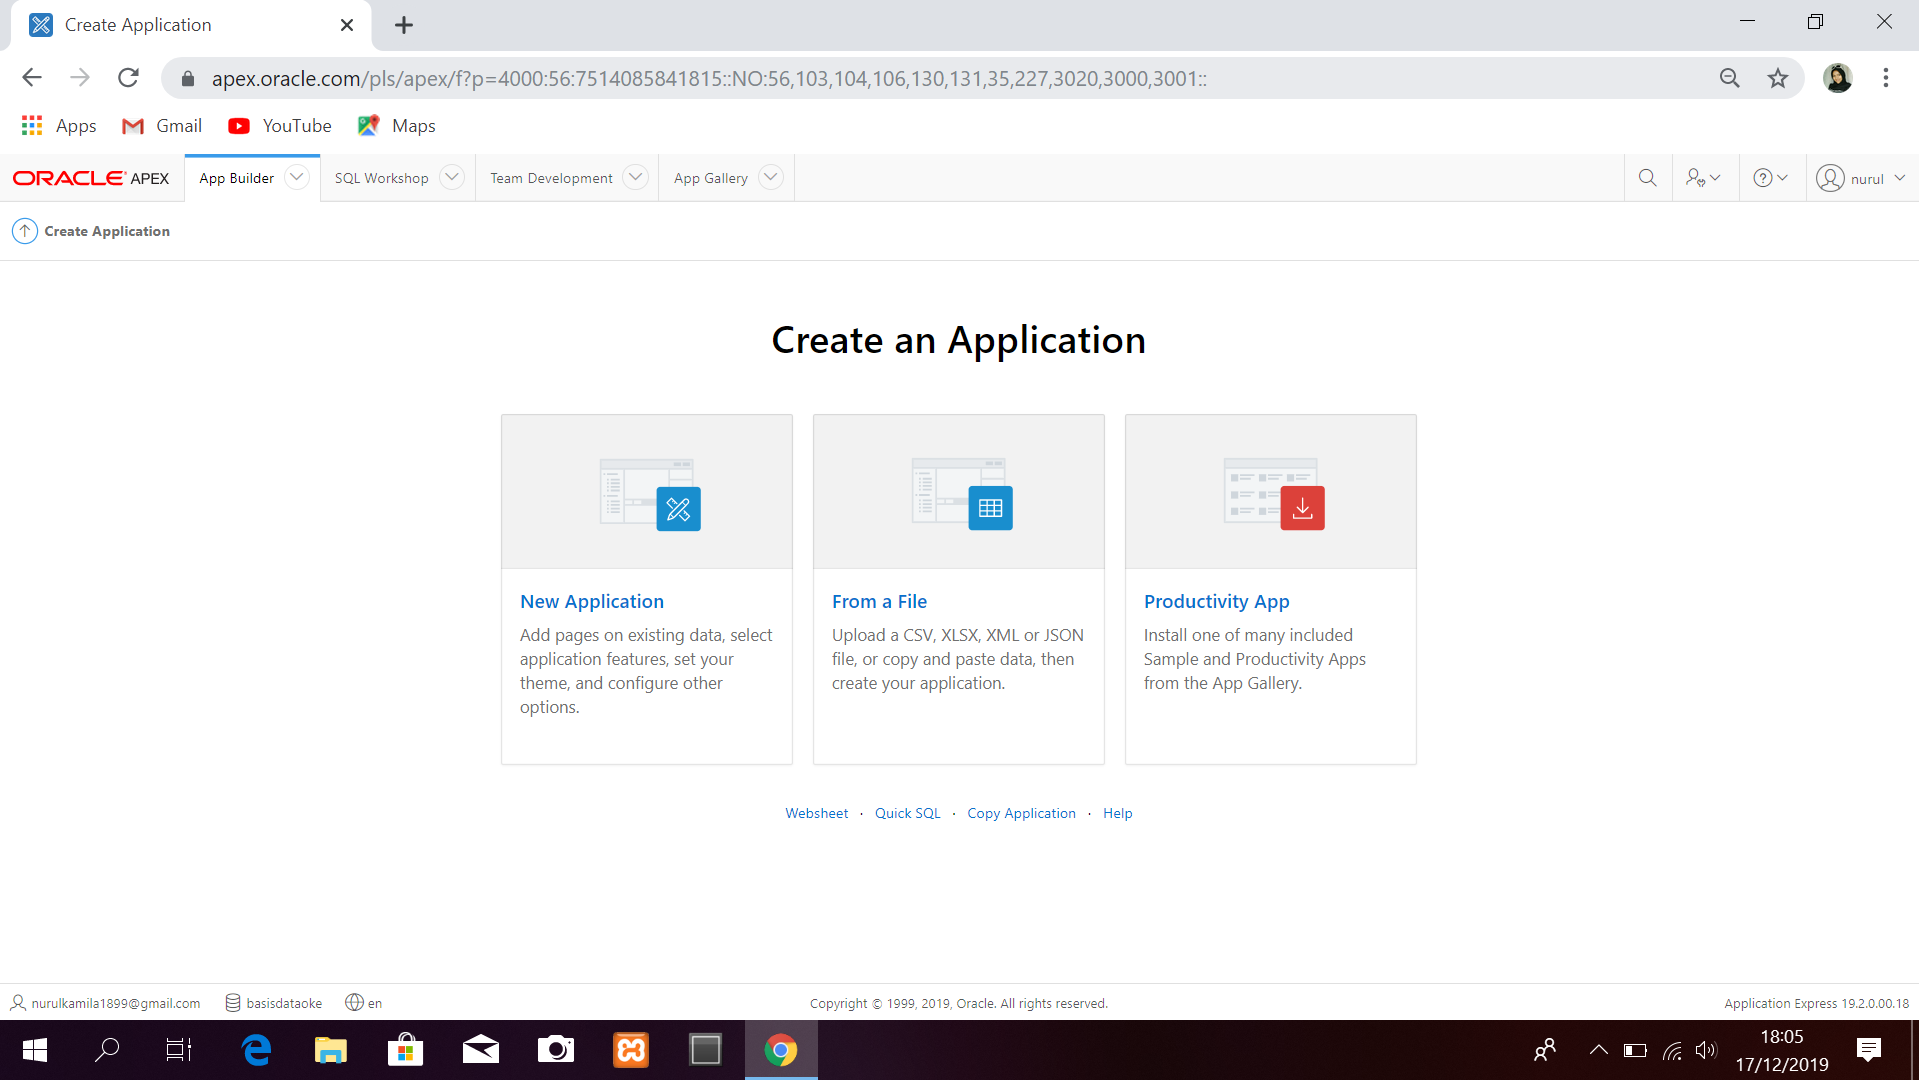
\includegraphics[width=.8\textwidth]{Figure/2.PNG}
     \end{center}
     
     \item  Lalu inputkan nama aplikasi yang akan kita buat
     \begin{center}
     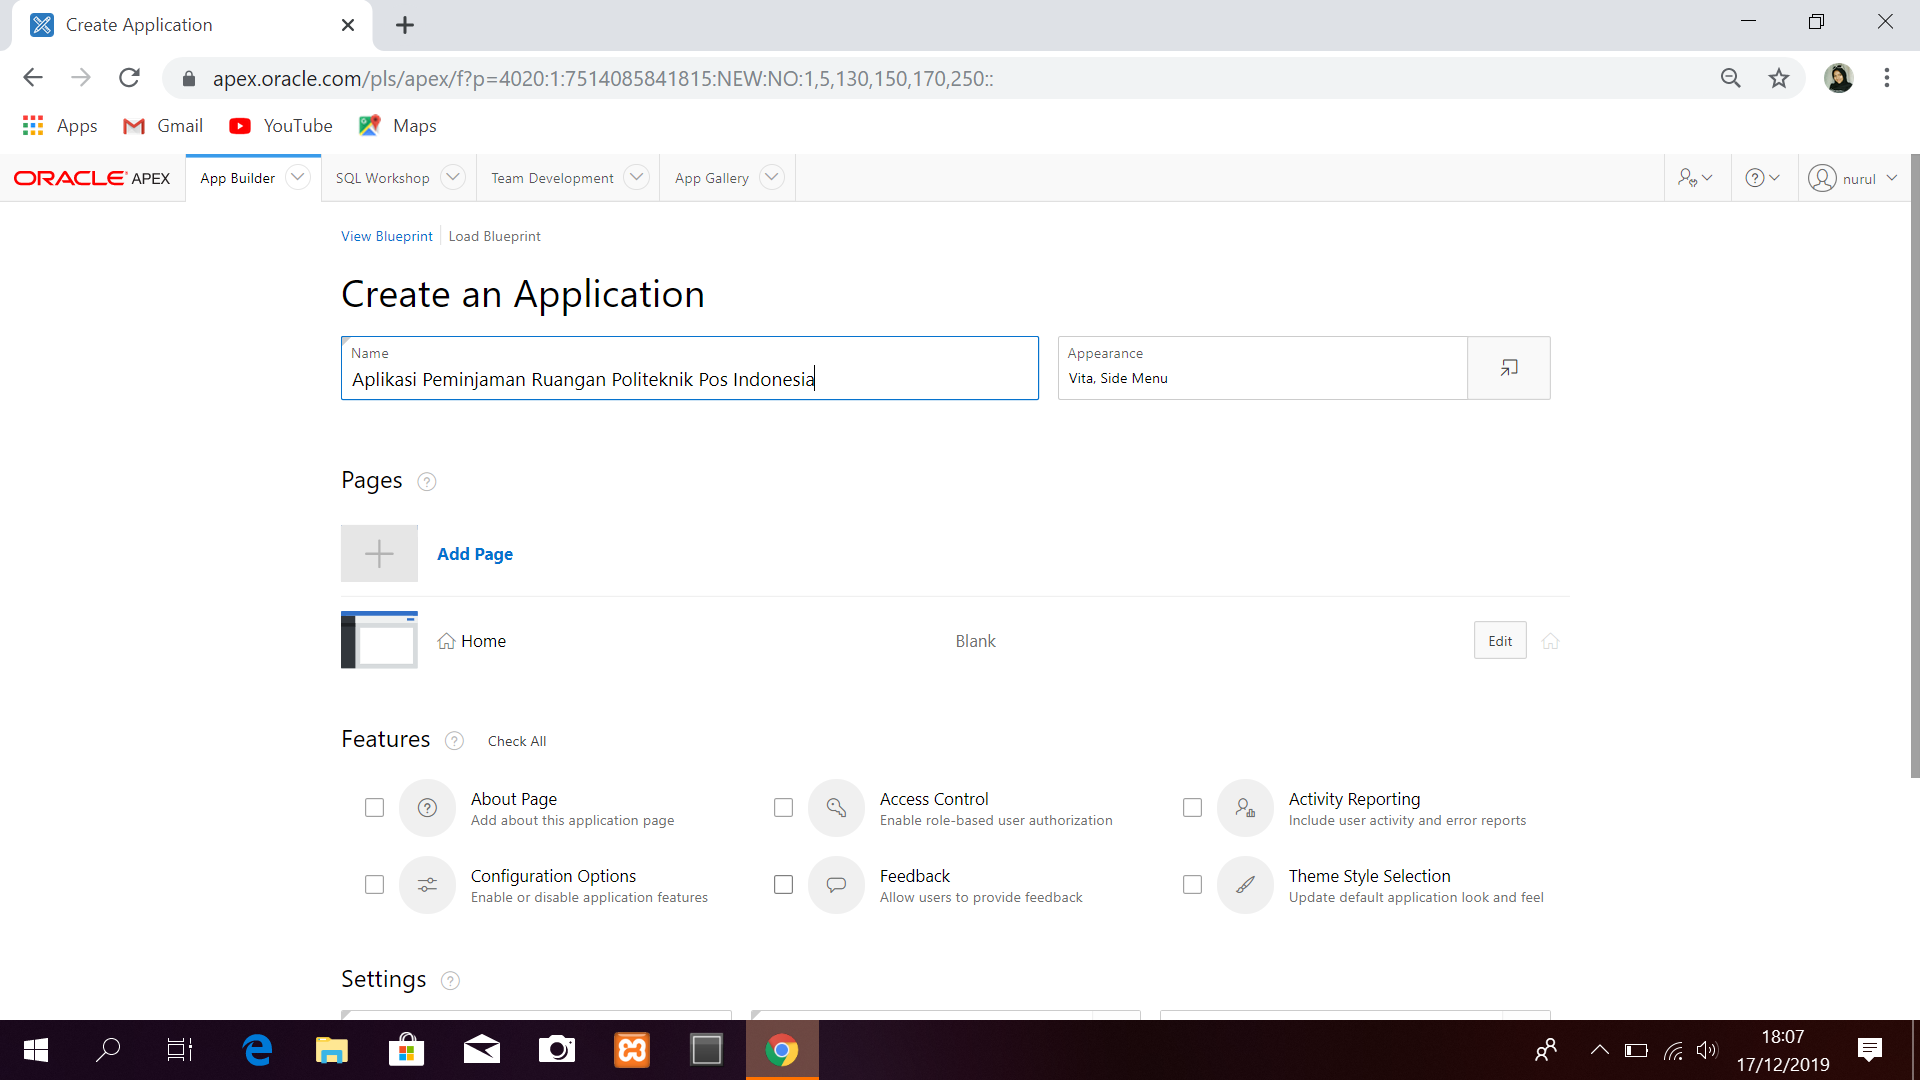
\includegraphics[width=.8\textwidth]{Figure/3.PNG}
     \end{center}
     
     \item  kemudian kita dapat memilih add page untuk menambahkan halaman-halaman baru dan tampilannya sesuai yang kita inginkan pada aplikasi kita. Disini saya menambahkan lima halaman baru yaitu halaman Mahasiswa yang akan menampilkan tabel Mahasiswa1 beserta datanya,  halaman BAAK yang akan menampilkan tabel BAAK beserta datanya, halaman Peminjaman yang akan menampilkan tabel Peminjaman beserta datanya, halaman Pembookingan ruangan yang akan menampilkan tabel View \textbf{PEMBOOKINGAN RUANGAN}, dan halaman Ruangan yang akan menampilkan tabel Ruang beserta datanya, seperti yang tertera pada gambar berikut:
     \begin{center}
     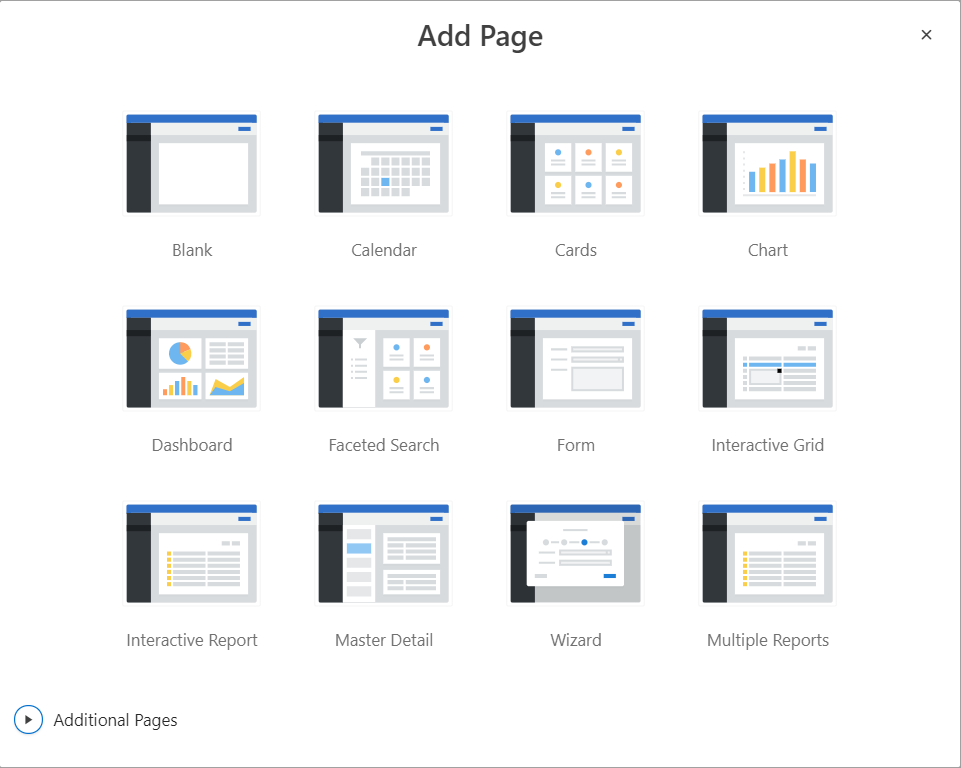
\includegraphics[width=.8\textwidth]{Figure/4.PNG}
     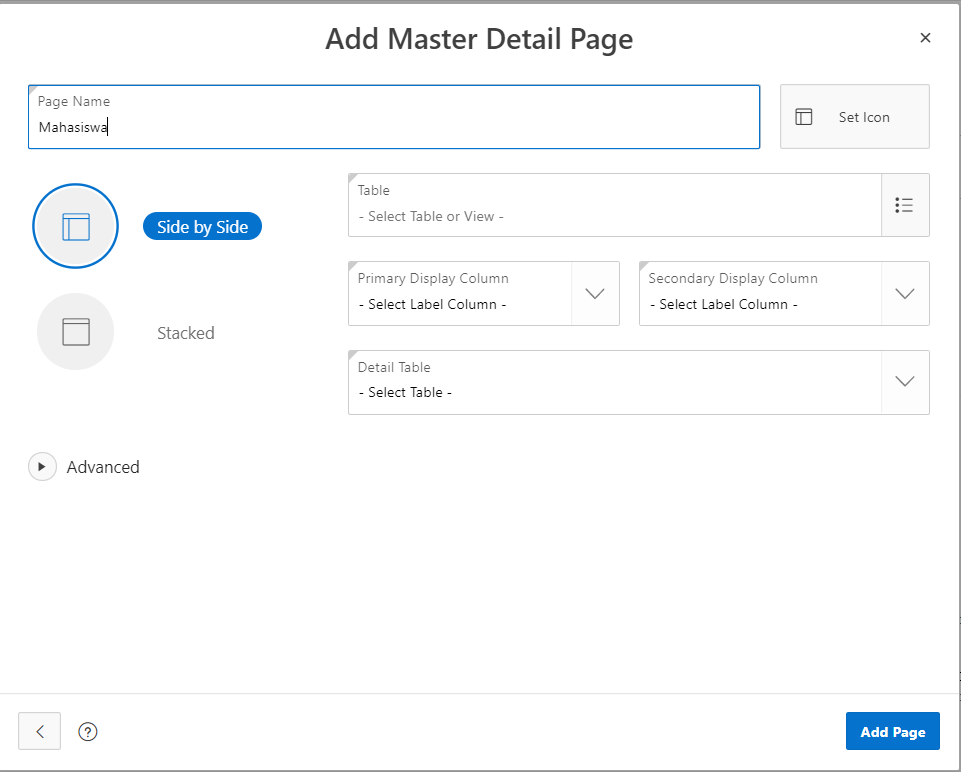
\includegraphics[width=.8\textwidth]{Figure/5.PNG}
     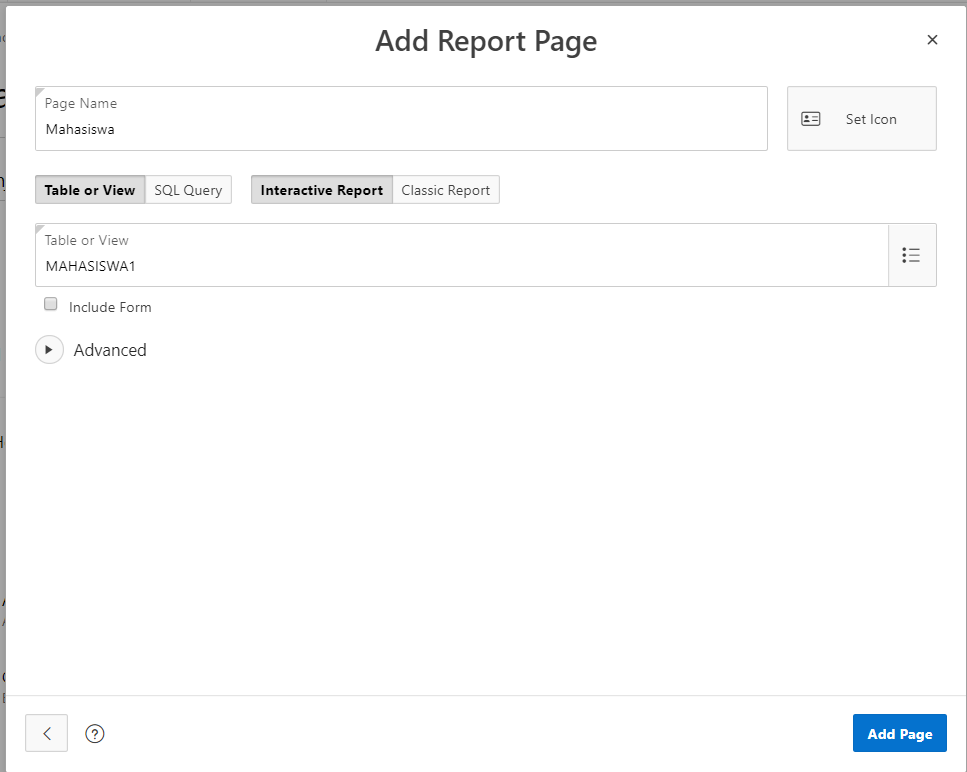
\includegraphics[width=.8\textwidth]{Figure/6.PNG}
     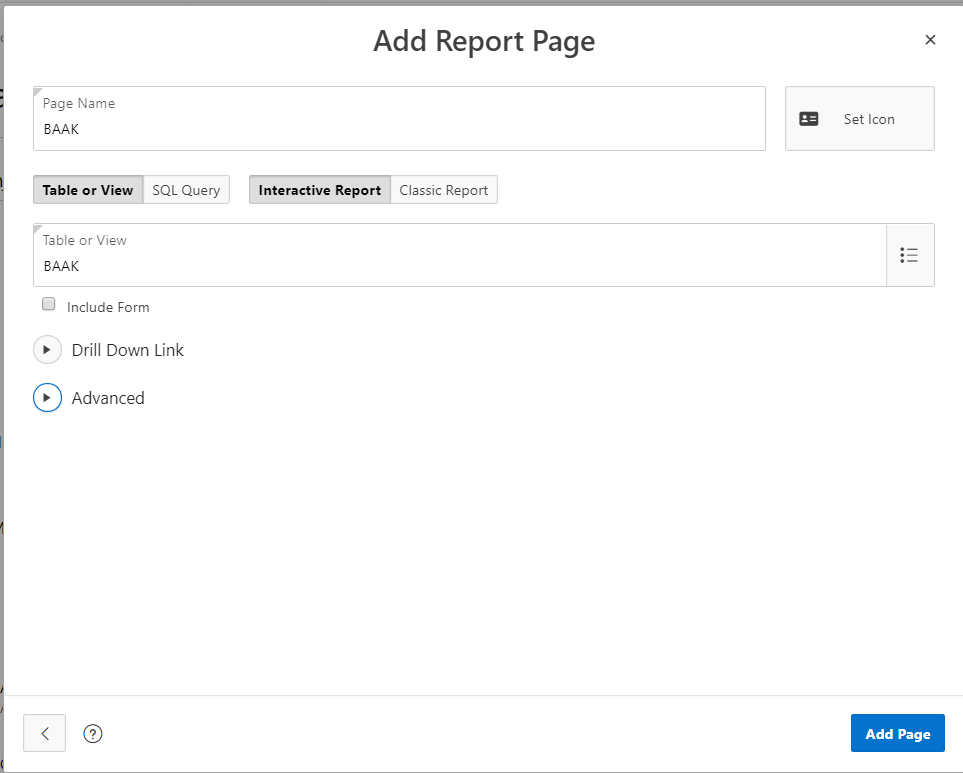
\includegraphics[width=.8\textwidth]{Figure/7.PNG}
     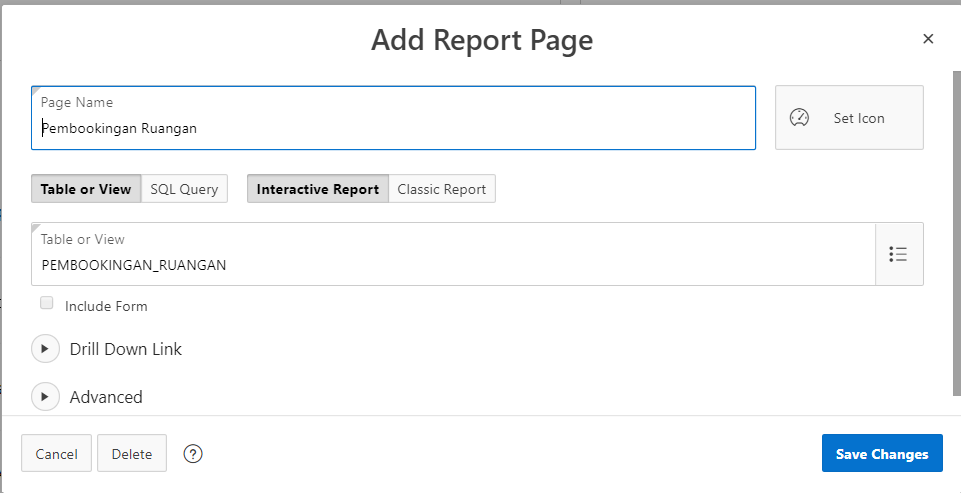
\includegraphics[width=.8\textwidth]{Figure/8.PNG}
     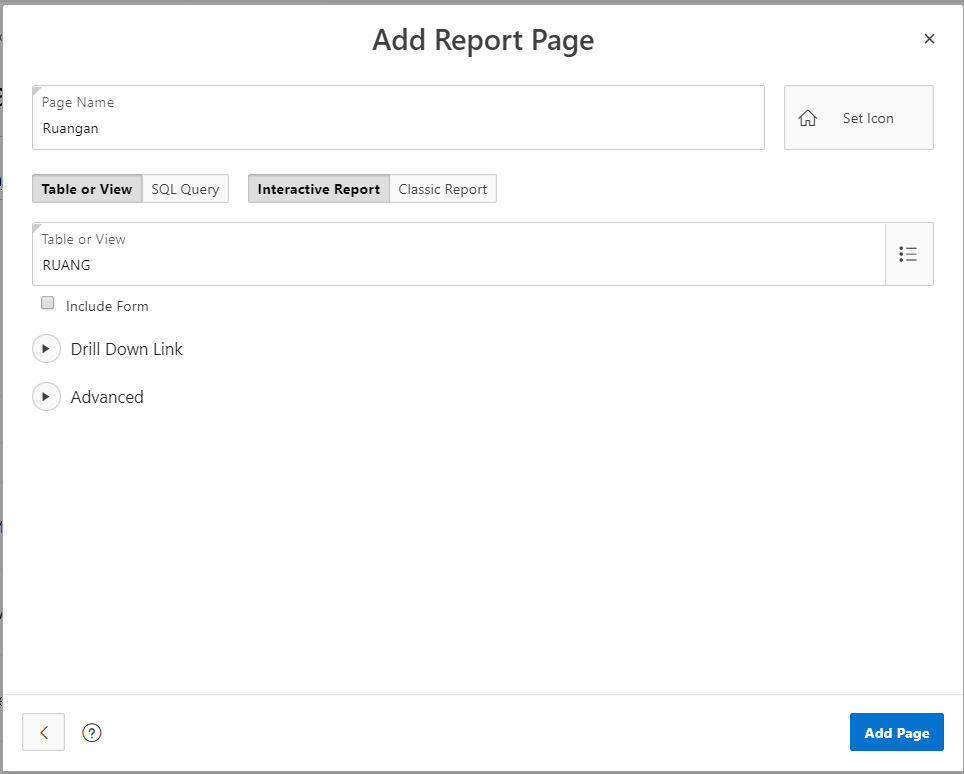
\includegraphics[width=.8\textwidth]{Figure/9.PNG}
     \end{center}
     
     \item  Setelah selesai membuat halaman-halaman tambahan pada aplikasi, lanjut ke menu Features yang terdapat di bawah Add Pages tadi, lalu centang semua pilihan yang terdapat pada Features tersebut, kemudian klik Create Application dan tunggu sampai loadingnya selesai.
     \begin{center}
     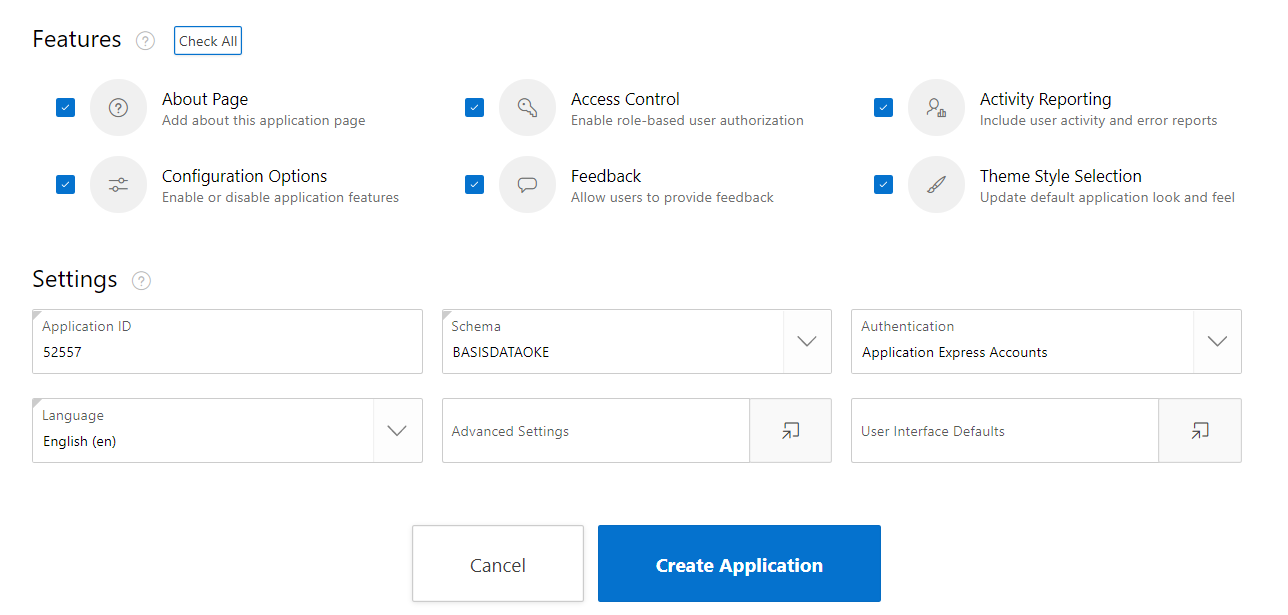
\includegraphics[width=.8\textwidth]{Figure/10.PNG}
     \end{center}
     
     \item Setelah berhasil dibuat aplikasinya, silahkan running aplikasi tersebut dengan memilih Run Application
     \begin{center}
     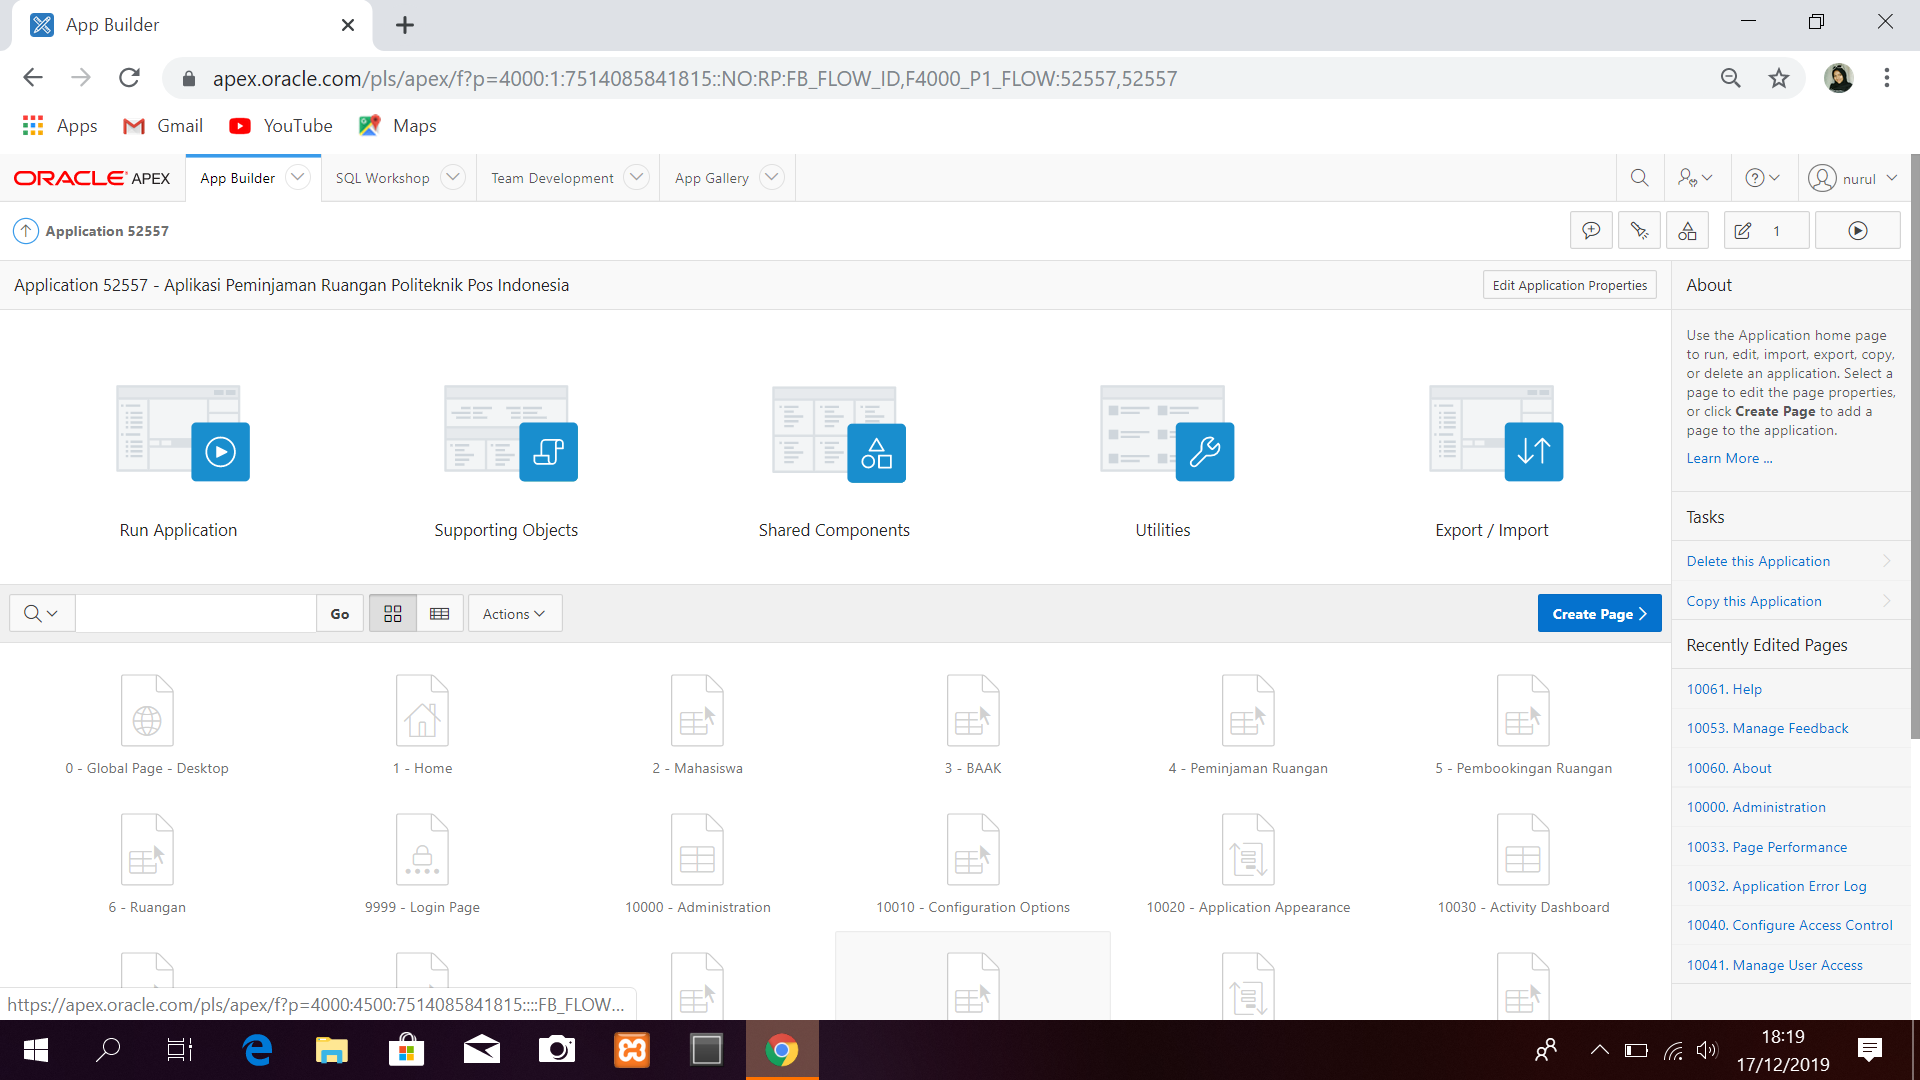
\includegraphics[width=.8\textwidth]{Figure/11.PNG}
     \end{center}\\
     
     Sebelum dijalankan kita akan disuruh menginputkan username dan password lagi 
     \begin{center}
     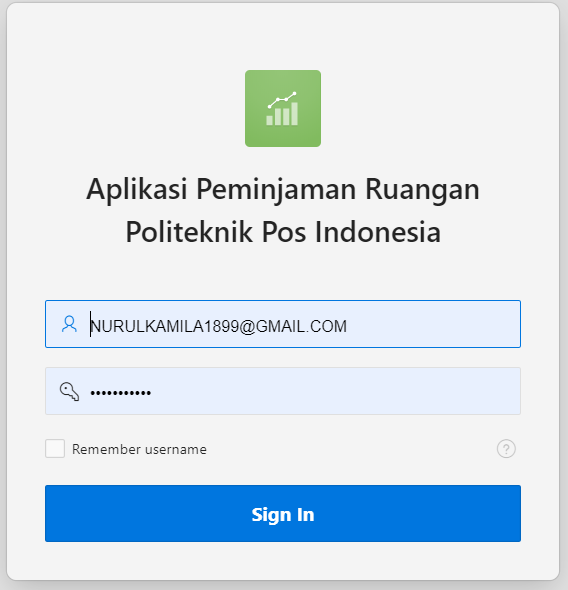
\includegraphics[width=.8\textwidth]{Figure/12.PNG}
     \end{center}
     
     \item  setelah Sign In kembali, maka kita sudah dapat membuka aplikasi yang kita buat 
     \begin{center}
     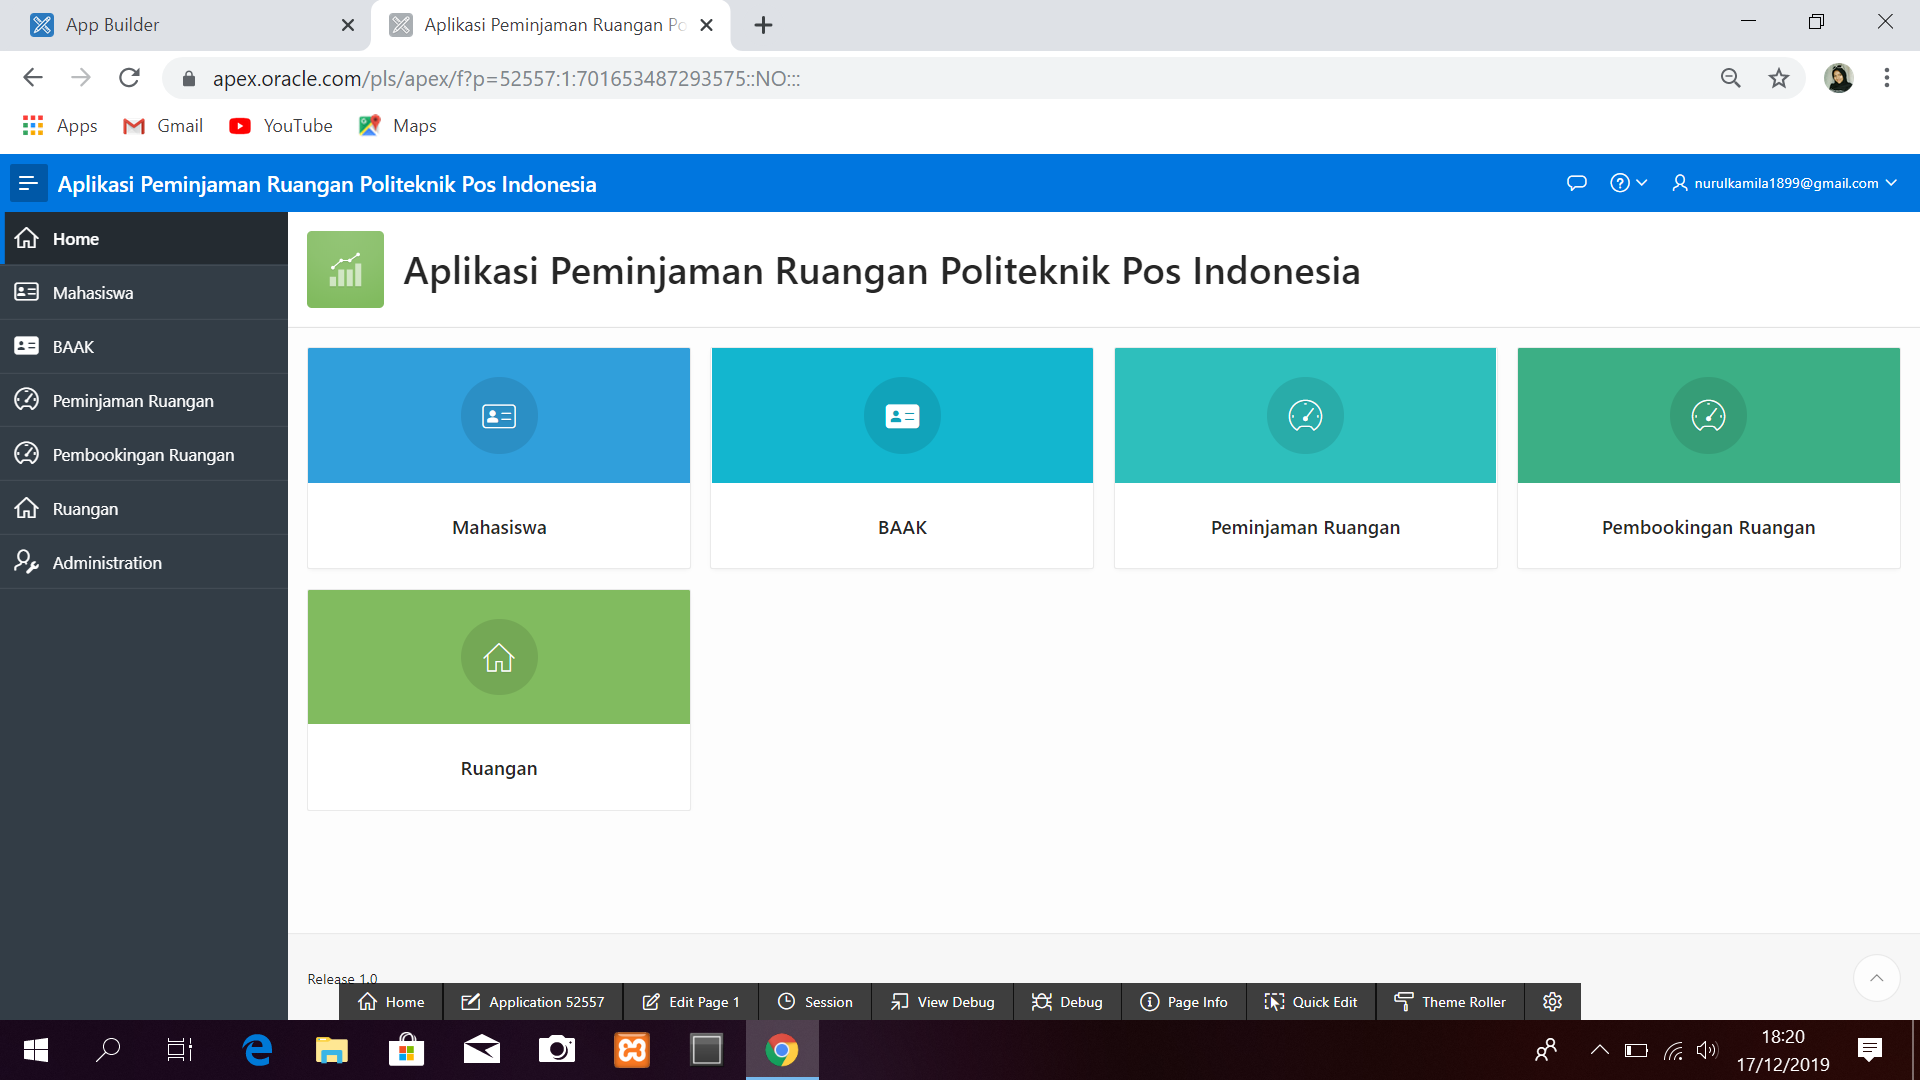
\includegraphics[width=.8\textwidth]{Figure/13.PNG}
     \end{center}\\
     \\
     
    https://apex.oracle.com/pls/apex/f?p=52557:LOGIN_DESKTOP:106726254303698:::::
    Username : NURULKAMILA1899@GMAIL.COM\\
    Password : twentytwo22

\end{enumerate}


\end{document}
